\documentclass{report}
\usepackage{mathtools}
\usepackage{unicode-math}
\usepackage{lualatex-math}
\usepackage{tcolorbox}
\setmainfont[
  BoldFont={STIXTwoText-Bold},
  ItalicFont={STIXTwoText-Italic},
  BoldItalicFont={STIXTwoText-BoldItalic}
]{STIXTwoText-Regular}
\setmathfont{STIXTwoMath-Regular}

\usepackage{mathdots}

\setlength{\parindent}{0pt}
\setlength{\parskip}{0.5em}

\usepackage{biblatex}
\addbibresource{references.bib}
\usepackage{amsmath}
\usepackage{listings}
\lstset{
  basicstyle=\ttfamily,
  mathescape
}

\renewcommand{\chaptername}{Poglavje}

\DeclareMathOperator{\acc}{symbol}

\usepackage{mathtools}
\usepackage{tikz}
\usetikzlibrary{automata, arrows.meta, positioning, arrows, fit, matrix, shapes.geometric, shapes.misc, calc}
\pgfdeclarelayer{background}
\pgfdeclarelayer{foreground}
\pgfsetlayers{background,main,foreground}

\newcounter{example}
%\newcommand{\N}[1]{{{#1}_{\arabic{example}}}}
\newcommand{\N}[1]{#1}
\newcommand{\Next}{\stepcounter{example}}
\newcommand{\Reset}{\setcounter{example}{1}}

\newcommand{\Ex}{\textbf{Npr.}:\ }
\newcommand{\Special}[1]{\textbf{#1}}
\newcommand{\Empty}{\varnothing}
\newcommand{\Null}{\varepsilon}
\newcommand{\Alphabet}{\Sigma}
\newcommand{\Language}[1]{\mathcal{L}(#1)}
\newcommand{\Automaton}[1]{\mathcal{M}(#1)}
\newcommand{\Str}[1]{\text{\textquotedbl\texttt{#1}\textquotedbl}}
\newcommand{\Char}[1]{\texttt{#1}}
\newcommand{\Seq}{\cdot}
\newcommand{\Pos}{\mathop{\mdsmblkcircle}}
\newcommand{\Spc}{\ }
\newcommand{\Union}{\mathrel{|}}
\newcommand{\Sum}{\mathrel{+}}
\newcommand{\Kleene}[1]{{#1}^\ast}
\newcommand{\Rep}[2]{{#1}^{#2}}
\newcommand{\Opt}[1]{#1?}
\newcommand{\KleenePlus}[1]{#1^+}
\newcommand{\Err}{\rdiagovfdiag}

\newcommand{\Set}[1]{\mathbf{#1}}

\newcommand{\FIRST}{\textsc{first}}
\newcommand{\FOLLOW}{\textsc{follow}}
\newcommand{\NEXT}{\textsc{next}}
\newcommand{\EOF}{\textsc{eof}}
\newcommand{\Terminals}{\Set{T}}
\newcommand{\Productions}{\Set{P}}
\newcommand{\NonTerminals}{\Set{N}}

\newcommand{\Arrow}{\Coloneq}
\newlength{\arrow}
\settowidth{\arrow}{\scriptsize$000$}
\newcommand{\MoveX}[1]{\xrightarrow{\mathmakebox[\arrow]{#1}}}
\newcommand{\Move}{\MoveX{}}
\newcommand{\Derive}{\Rightarrow}
\newcommand{\DeriveStar}{\Rightarrow^\ast}
\newcommand{\DerivePlus}{\Rigtharrow^+}

\newcommand{\NT}[1]{{#1}}
\newcommand{\T}[1]{{#1}}
\newcommand{\Var}[1]{{#1}}
\newcommand{\Sym}[1]{{#1}}
\newcommand{\RE}[1]{{#1}}
\newcommand{\Lookahead}[1]{{}_{\{{#1}\}}}

\makeatletter
\DeclareRobustCommand{\Dots}{%
  \vbox{
    \baselineskip4\p@\lineskiplimit\z@
    \kern-\p@
    \hbox{.}\hbox{.}\hbox{.}
  }}
\makeatother

\lstnewenvironment{algorithm}[1][]
{
    \lstset{
        mathescape=true,
        %frame=tB,
        numbers=left, 
        %numberstyle=\tiny,
        basicstyle=\footnotesize, 
        %keywordstyle=\color{black}\bfseries\em,
        keywords={,input, output, return, datatype, function, in, if, else, foreach, while, begin, end, } 
        numbers=left,
        xleftmargin=.04\textwidth,
        #1
    }
}
{}

\tikzset{
    cross/.pic = {
    \draw[rotate = 45] (-#1,0) -- (#1,0);
    \draw[rotate = 45] (0,-#1) -- (0, #1);
    },
    hide/.style={draw=none, fill=none},
    ellip/.append style={ellipse, inner sep=-0.14cm},
    every state/.append style={font=\footnotesize},
}

\begin{document}

\chapter{Končni avtomati}

\section{Jezik}
Jezik je (ne nujno končna) množica nizov.

\Ex
\begin{equation*}
  L = \{\Str{}, \Str{DoberDan}, \Str{123}, \Str{/}, \Str{1 + 1} \}
\end{equation*}

\section{Regularni izrazi}
Regularni izrazi so algebra nad jeziki, ki sestavljena iz osnovnih operacij $(\Union)$, $(\Seq)$, $(\ast)$ in osnovnih elementov $\Char{a}$, $\Empty$, $\Null$.
Z njimi lahko opišemo le podmnožico vseh jezikov, ki se imenuje "regularni jeziki".
Dva regularna izraza sta enaka, če opisujeta enak jezik.

\section{Končni avtomati}

Končni avtomat je tuple $(Q, \Alphabet, \delta, q_0, F)$, kjer je $Q$ končna množica stanj, $\Sigma$ končna množica znakov ali abeceda, $\delta$ je funkcija prehodov in $F$ končna množica končnih stanj.
Tuple lahko implementiramo kot \emph{struct} ali \emph{record}.
Funkcija prehodov ima signaturo $Q \times \Sigma \not\rightarrow Q$.
Implementiramo jo lahko, kot asociativni seznam, iskalno drevo ali tabelo.

\Special{Meta:} Avtomat regularnega izraza $r$ bo označen kot $\Automaton{r}$.

\Special{Meta:} Simbol $\Err$ označuje neveljavno stanje.

\Ex
\begin{equation}
  r_1 = \Kleene{(\Char{b} \Seq (\Char{a} \Spc \Char{b})?)} \Seq \Char{c} \\
\end{equation}
\begin{align*}
  \Automaton{r_1} &= (Q_1, \Sigma, \delta_1, q_{0, 1}, F_1)\\[1em]
  Q_1 &= \{1, 2, 3\} \\[1em]
  \Sigma &= \{\Char{a}, \Char{b}, \Char{c}\} \\[1em]
  \delta_1(1, \Char{b}) & =  2\\
  \delta_1(2, \Char{a}) & =  1\\
  \delta_1(2, \Char{b}) & =  2\\
  \delta_1(2, \Char{b}) & =  3\\[1em]
  q_{0, 1} &= 1 \\[1em]
  F_1 &= \{3\}
\end{align*}

\begin{center}
\begin{tabular}{ | c | c | c | c | }
   \hline
   $\delta_1$ & \Char{a} & \Char{b} & \Char{c} \\
   \hline
  1 & $\Err$ & 2 & $\Err$  \\
   \hline
  2 & 1 & 2 & 3  \\
   \hline
  3 & $\Err$ & $\Err$ & $\Err$   \\
   \hline
\end{tabular}
\end{center}

\begin{center}
  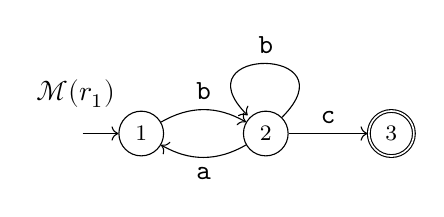
\begin{tikzpicture}
    \tikzset{
      node distance=1cm,
      every state/.append style={minimum size=0.5cm},
      initial text=$ $
    }

    \node[state, initial, label=above left:$\Automaton{r_1}$] (s0) {1};
    \node[state, right=of s0] (s1) {2};
    \node[state, accepting, right=of s1] (s2) {3};

    \draw (s0) edge[->, bend left] node[auto]{$\Char{b}$} (s1);
    \draw (s1) edge[->, bend left] node[auto]{$\Char{a}$} (s0);
    \draw (s1) edge[->, loop] node[above]{$\Char{b}$} (s1);
    \draw (s1) edge[->] node[auto]{$\Char{c}$} (s2);
  \end{tikzpicture}
\end{center}

\Ex

Vsak regularni izraz lahko ustreza večim različnim avtomatom.

\begin{gather*}
  r_2 = \Kleene{(\Char{b} \Seq (\Char{a} \Spc \Char{b})?)} \Seq \Char{c} \\
  \Automaton{r_2} = (Q_2, \Sigma, \delta_2, q_{0, 2}, F_2)
\end{gather*}

\begin{center}
  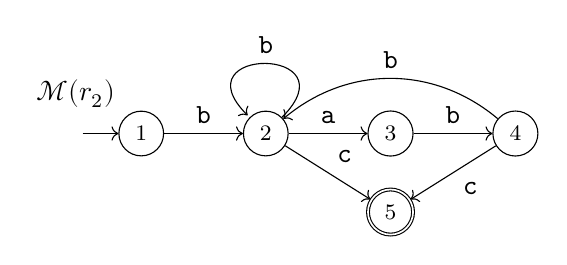
\begin{tikzpicture}
    \tikzset{
      node distance=1cm,
      every state/.append style={minimum size=0.5cm},
      initial text=$ $
    }

    \node[state, initial, label=above left:$\Automaton{r_2}$] (s0) {1};
    \node[state, right=of s0] (s1) {2};
    \node[state, right=of s1] (s2) {3};
    \node[state, right=of s2] (s3) {4};
    \node[state, accepting, below=0.4cm of s2] (s4) {5};

    \draw (s0) edge[->] node[auto]{$\Char{b}$} (s1);
    \draw (s1) edge[->, loop] node[above]{$\Char{b}$} (s1);
    \draw (s1) edge[->] node[auto]{$\Char{a}$} (s2);
    \draw (s2) edge[->] node[auto]{$\Char{b}$} (s3);
    \draw (s1) edge[->] node[auto]{$\Char{c}$} (s4);
    \draw (s3) edge[->] node[auto]{$\Char{c}$} (s4);
    \draw (s3) edge[->, bend right=40] node[above]{$\Char{b}$} (s1);
  \end{tikzpicture}
\end{center}

Funkcijo prehodov lahko definiramo tudi za niz:
\begin{align*} % XXX define empty string
  \Kleene{\delta}(q, \varepsilon) &= q\\
  \Kleene{\delta}(q, a \Seq w) &= \Kleene{\delta}(q', w) \text{, kjer } q' = \delta(q, a) \text{ in } q' \neq \Err
\end{align*}

\Ex
\begin{align*}
  \Kleene{\delta_1}(1, \Str{b}) &= 2 \\
  \Kleene{\delta_1}(1, \Str{ba}) &= 1 \\
  \Kleene{\delta_1}(1, \Str{bab}) &= 2 \\
  \Kleene{\delta_1}(1, \Str{bc}) &= 3 \\
  \Kleene{\delta_1}(1, \Str{babbc}) &= 3 \\
  \Kleene{\delta_1}(2, \Str{bbb}) &= 2 \\
  \Kleene{\delta_1}(2, \Str{abbc}) &= 3
\end{align*}

Jezik, ki ga avtomat opisuje:
\begin{equation*}
  L = \{w \in \Kleene{\Sigma} \mid \Kleene{\delta}(q_0, w) \in F\}
\end{equation*}

\Ex

\begin{align*}
  \Kleene{\delta_1}(1, \Str{bc}) &= 3 \\
  \Kleene{\delta_1}(1, \Str{bbc}) &= 3 \\
  \Kleene{\delta_1}(1, \Str{bbbc}) &= 3 \\
  \cdots \\
  \Kleene{\delta_1}(1, \Str{babc}) &= 3 \\
  \Kleene{\delta_1}(1, \Str{bababc}) &= 3 \\
  \ldots \\
  \Kleene{\delta_1}(1, \Str{babbc}) &= 3 \\
  \Kleene{\delta_1}(1, \Str{babbbc}) &= 3 \\
  \cdots \\
  \Kleene{\delta_1}(1, \Str{bababbc}) &= 3 \\
  \Kleene{\delta_1}(1, \Str{bababbbc}) &= 3 \\
  \cdots \\
\end{align*}

\begin{multline*}
  L = \{ \Str{bc}, \Str{bbc}, \Str{bbbc}, \ldots, \Str{babc}, \Str{bababc}, \ldots,\\
  \Str{babbc},  \Str{babbbc}, \ldots, \Str{bababbc}, \Str{bababbbc}, \dots \}
\end{multline*}

%Za implementacijo pregledovalnika je potrebno končnemu avtomatu dodati funkcijo, ki končna stanja preslika v terminale:
%\begin{equation*}
%  \acc: Q \rightarrow T
%\end{equation*}

\section{Konstrukcija}

Trenutna pozicija $\Pos$.

\begin{equation*}
  \begin{aligned}
    \Pos\Empty &\Move \Empty
  \end{aligned}
\end{equation*}

\begin{equation*}
  \begin{aligned}
    \Pos\Null &\Move \Null\Pos
  \end{aligned}
\end{equation*}

\begin{equation*}
  \begin{aligned}
    \Pos\Char{a} &\MoveX{\Char{a}} \Char{a}\Pos\\
    (\RE{R})\Pos &\MoveX{\Char{a}} \RE{R}\\
    \Pos\Char{a} &\MoveX{\Char{b}} \Char{a}
  \end{aligned}
\end{equation*}

\begin{equation*}
  \begin{aligned}
    \Pos(\RE{R} \Seq \RE{S}) &\Move (\Pos\RE{R}) \Seq \RE{S}\\
    (\RE{R}\Pos) \Seq \RE{S} &\Move \RE{R} \Seq (\Pos \RE{S})\\
    \RE{R} \Seq (\RE{S} \Pos) &\Move (\RE{R} \Seq \RE{S})\Pos
  \end{aligned}
\end{equation*}

\begin{equation*}
  \begin{aligned}
    \Pos(\RE{R} \Union \RE{S}) &\Move (\Pos\RE{R}) \Union (\Pos\RE{S})\\
    (\RE{R}\Pos) \Union \RE{S} &\Move (\RE{R} \Union \RE{S})\Pos\\
    \RE{R} \Union (\RE{S}\Pos) &\Move (\RE{R} \Union \RE{S})\Pos
  \end{aligned}
\end{equation*}

\begin{equation*}
  \begin{aligned}
    \Pos(\RE{R}?) &\Move ((\Pos\RE{R})?)\Pos\\
    (\RE{R}\Pos)? &\Move (\RE{R}?)\Pos
  \end{aligned}
\end{equation*}

\begin{equation*}
  \begin{aligned}
    \Pos(\RE{R}+) &\Move (\Pos\RE{R})+\\
    (\RE{R}\Pos)+ &\Move ((\Pos\RE{R})+)\Pos
  \end{aligned}
\end{equation*}

\begin{equation*}
  \begin{aligned}
    \Pos(\Kleene{\RE{R}}) &\Move (\Kleene{(\Pos\RE{R})})\Pos\\
    \Kleene{(\RE{R}\Pos)} &\Move (\Kleene{(\Pos\RE{R})})\Pos
  \end{aligned}
\end{equation*}

\begin{center}
  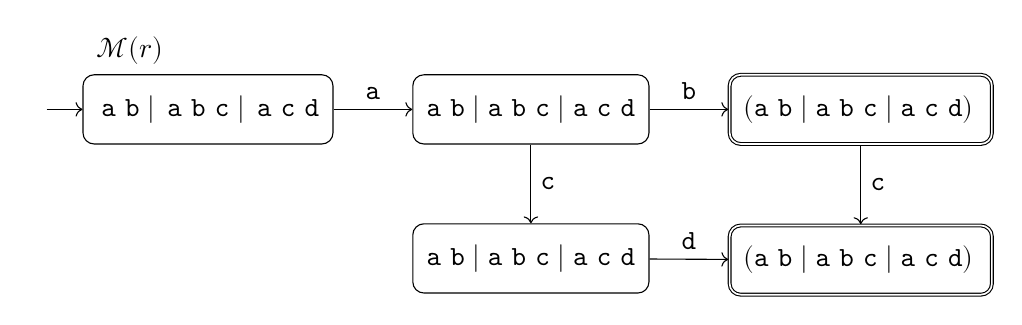
\begin{tikzpicture}
    \tikzset{
      node distance=1cm,
      %every state/.append style={minimum size=0.5cm},
      every state/.style={rectangle, rounded corners, inner sep=0.5em},
      initial text=$ $,
      large/.style={minimum size=1.5cm},
    }

    \node[state, initial, label=above left:$\Automaton{r}$] (u0) {$\Pos\Char{a} \Spc \Char{b} \Union \Pos\Char{a}\Spc\Char{b}\Spc\Char{c} \Union \Pos\Char{a}\Spc\Char{c}\Spc\Char{d}$};
    \node[state, right=of u0] (u1) {$\Char{a} \Pos\Char{b} \Union \Char{a}\Pos\Char{b}\Spc\Char{c} \Union \Char{a}\Pos\Char{c}\Spc\Char{d}$};
    \node[state, accepting, right=of u1] (u2) {$(\Char{a} \Spc\Char{b} \Union \Char{a}\Spc\Char{b}\Pos\Char{c} \Union \Char{a}\Spc\Char{c}\Spc\Char{d})\Pos$};
    \draw (u0) edge[->] node[auto]{$\Char{a}$} (u1);
    \draw (u1) edge[->] node[auto]{$\Char{b}$} (u2);

    \node[state, below=of u1] (u4) {$\Char{a} \Spc\Char{b} \Union \Char{a}\Spc\Char{b}\Spc\Char{c} \Union \Char{a}\Spc\Char{c}\Pos\Char{d}$};
    \node[state, accepting, below=of u2] (u3) {$(\Char{a} \Spc\Char{b} \Union \Char{a}\Spc\Char{b}\Spc\Char{c} \Union \Char{a}\Spc\Char{c}\Spc\Char{d})\Pos$};

    \draw (u2) edge[->] node[auto]{$\Char{c}$} (u3);
    \draw (u1) edge[->] node[auto]{$\Char{c}$} (u4);
    \draw (u4) edge[->] node[auto]{$\Char{d}$} (u3);
  \end{tikzpicture}
\end{center}


\end{document}
